\documentclass[dvipsnames]{beamer}

\usepackage{xcolor}
\usepackage{lmodern}
\usepackage{minted}
\usepackage[utf8]{inputenc}
\usepackage{standalone}
\usepackage{tikz}
\usepackage{caption}
\usepackage{adjustbox}
\usepackage{upquote}
\usepackage{hyperref}
\usepackage{multirow}
\usepackage{booktabs}
\usepackage{array}
\usepackage{xspace}
\usetikzlibrary{mindmap,shadows,arrows,positioning,chains,fit,shapes}

\usetheme{metropolis}
\usemintedstyle{manni}

\definecolor{gmitblue}{RGB}{20,134,225}
\definecolor{gmitred}{RGB}{220,20,60}
\definecolor{gmitgrey}{RGB}{67,67,67}

\setbeamercolor{structure}{fg=gmitblue}
\setbeamercolor{frametitle}{fg=white,bg=gmitred}
\setbeamercolor{alerted text}{fg=gmitblue}

\renewcommand\footnoterule{}
\newcommand{\citeurl}[1]{\let\thefootnote\relax\footnotetext{\tiny \textcolor{gmitgrey}{\href{http://#1}{#1}}}}

\begin{document}
  %!TEX root = slides.tex

\title{Module title}
\subtitle{}
\author{ian.mcloughlin@gmit.ie}
\date{}


\begin{frame}
  \titlepage
\end{frame}

\begin{frame}{Topics}
  \tableofcontents
\end{frame}


\section{First topic}

\begin{frame}{About stuff}
  \metroset{block=fill}
  \begin{alertblock}{Stuff}
  Cool.
  \end{alertblock}
\end{frame}

\section{Second topic}

\begin{frame}[fragile]{Code}
  \begin{minted}{python}
x = int(raw_input("Please enter an integer: "))
if x < 0:
  x = 0
  print 'Negative changed to zero'
elif x == 0:
  print 'Zero'
elif x == 1:
  print 'Single'
else:
  print 'More'
  \end{minted}
  \citeurl{docs.python.org/2/tutorial}
\end{frame}

\section{Section three}

\begin{frame}{John McCarthy}
  \begin{columns}
    \begin{column}{1.5in}
      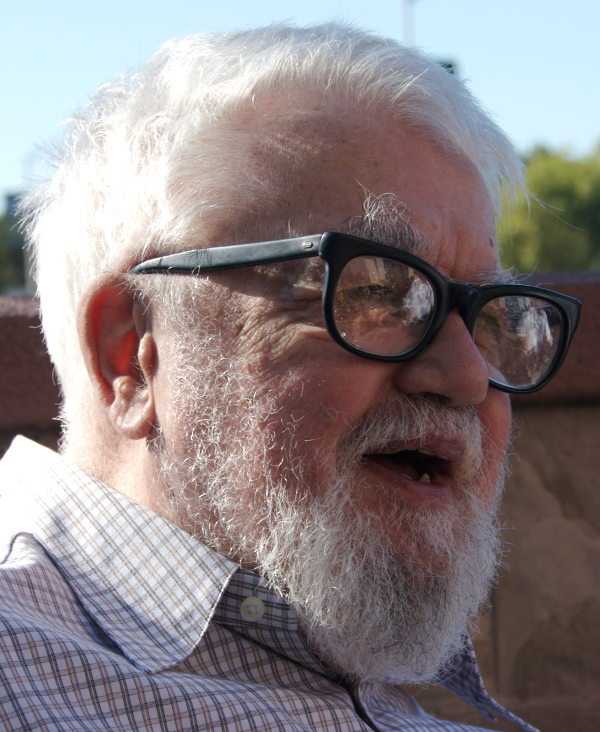
\includegraphics[width=1.4in]{img/john-mccarthy.png}
    \end{column}
    \begin{column}{0.7\textwidth}
      \begin{itemize}
        \item John McCarthy while at MIT -- late 1950s.
        \vspace{0.25cm}
        \item Created Lisp.
        \vspace{0.25cm}
        \item Lisp generally considered first functional programming language (not really though).
        \vspace{0.25cm}
        \item Lots of dialects exist today, such as Scheme and Common Lisp.
      \end{itemize}
    \end{column}
  \end{columns}
  \citeurl{www-formal.stanford.edu/jmc/}
\end{frame}


\section{Section four}


\begin{frame}{Turing Machine}
  \begin{adjustbox}{max width={0.9\textwidth},center} 
  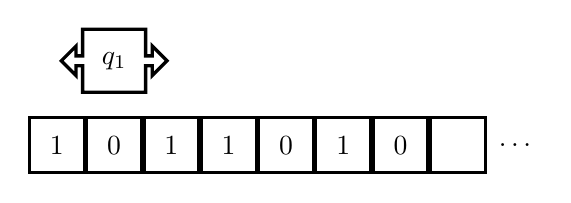
\begin{tikzpicture}
  \tikzstyle{every path}=[very thick]
  
  \edef\sizetape{0.7cm}
  \tikzstyle{tmtape}=[draw,minimum size=\sizetape]
  \tikzstyle{tmhead}=[arrow box,draw,minimum size=.8cm,arrow box arrows={east:.25cm, west:0.25cm}]
  
  \begin{scope}[start chain=1 going right,node distance=-0.15mm]
  \node [on chain=1,tmtape] {1};
  \node [on chain=1,tmtape] (input) {0};
  \node [on chain=1,tmtape] {1};
  \node [on chain=1,tmtape] {1};
  \node [on chain=1,tmtape] {0};
  \node [on chain=1,tmtape] {1};
  \node [on chain=1,tmtape] {0};
  \node [on chain=1,tmtape] {};
  \node [on chain=1,tmtape,draw=none] {$\ldots$};
  \end{scope}

  \node [tmhead,yshift=.7cm] at (input.north) (head) {$q_1$};
  \end{tikzpicture}
  \end{adjustbox}

  \vspace{1.5cm}

  \begin{adjustbox}{max width={0.9\textwidth},center} 
    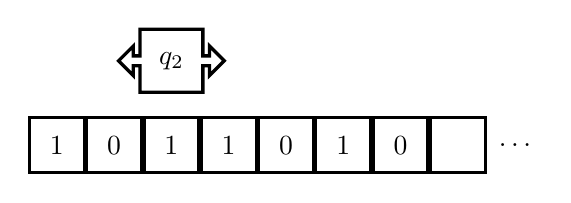
\begin{tikzpicture}
    \tikzstyle{every path}=[very thick]
    
    \edef\sizetape{0.7cm}
    \tikzstyle{tmtape}=[draw,minimum size=\sizetape]
    \tikzstyle{tmhead}=[arrow box,draw,minimum size=.8cm,arrow box arrows={east:.25cm, west:0.25cm}]
    
    \begin{scope}[start chain=1 going right,node distance=-0.15mm]
    \node [on chain=1,tmtape] {1};
    \node [on chain=1,tmtape] {0};
    \node [on chain=1,tmtape] (input) {1};
    \node [on chain=1,tmtape] {1};
    \node [on chain=1,tmtape] {0};
    \node [on chain=1,tmtape] {1};
    \node [on chain=1,tmtape] {0};
    \node [on chain=1,tmtape] {};
    \node [on chain=1,tmtape,draw=none] {$\ldots$};
    \end{scope}
    
    \node [tmhead,yshift=.7cm] at (input.north) (head) {$q_2$};
    \end{tikzpicture}
  \end{adjustbox}
\end{frame}

\begin{frame}{State Table}
  \begin{table}
    \centering
    \begin{tabular}{cc|ccc}
      \toprule
      State  & Input  & Write & Move & Next \\
      \midrule
      \multirow{3}{*}{0} 
      & B & B &  & Accept \\
      & 0 & 0 & L & 0 \\
      & 1 & 1 & L & 1 \\
      \midrule
      \multirow{3}{*}{1}
      & B & B &  & Fail \\
      & 0 & 0 & L & 1 \\
      & 1 & 1 & L & 0 \\
      \bottomrule
    \end{tabular}
  \end{table}
  
  \[ \delta(q_i, g_n) \rightarrow (q_j, g_m, L/R) \]
\end{frame}

\end{document}